\section{Android app}
\label{sec:arch_app}
The app is developed to run on Android versions 4.0 or greater. As of March 2014 this makes up for 79,7\% of all Android devices in use~\cite{AndroidDeviceFragmentation}.
Support for earlier versions would require extra work, and because the app is a proof-of-concept this was not considered a problem.

The best practice guidelines for Android~\cite{androidPracticePerformance} state that one should avoid using a complex architecture. A complex architecture will increase the code base and is unnecessary in most situations. A structured pattern with concise code guidelines is needed to keep the development process as simple, effective, and bug free as possible. This section will give a detailed description of the Android app architecture. 

\subsection{Overall structure}
The Activity is the starting point of the app. It is a self contained process with the possibility to display a user interface to the user.

To access the different parts of the app it was decided to use a ~\gls{navigation drawer}. The sections accessed through the navigation drawer is called a tab. 

The navigation drawer and all of the tabs are implemented as Fragments. A Fragment is a representation of some behavior or an interface. It is embedded inside an Activity and can be swapped in and out of the Activity. Multiple Fragments can live in the same view. A subset of the Activity life-cycle is implemented in Fragments so it can work as a self-contained module. To read more about the Android life-cycle, see the official Android documentation.~\cite{androiddoc}

The navigation drawer handles when a tab is clicked. A callback to the main activity is issued, and the Fragment view is swapped in.

Each tab has its own logic and has a default behavior defined by 'DefaultTabFragment`. A class diagram illustrating the main Fragments is shown in figure~\ref{fig:classDiagramFragments}. The default behavior takes care of updating the name of the current tab to the Action Bar.

\begin{figure}[H]
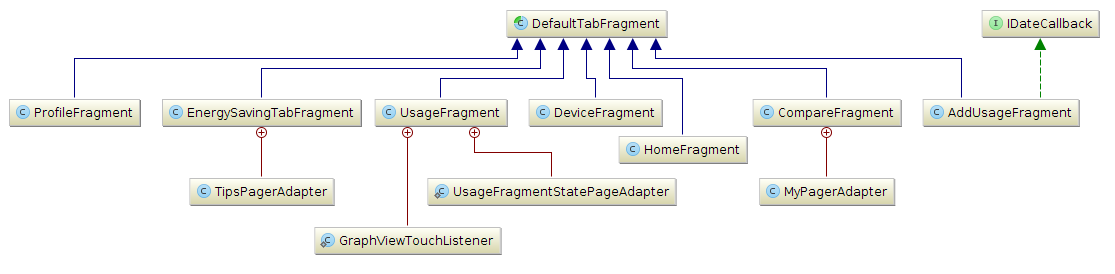
\includegraphics[width=\textwidth]{ch/architecture/fig/class_diagram_fragments.png}
\caption{Class diagram for the fragments.}
\label{fig:classDiagramFragments}
\end{figure}

\subsection{Android rendering and the main thread}
One of the key issues on mobile app development (besides having a good interface design) is keeping the \gls{UI} responsive. Having a UI that lags will most often upset the user and result in the app being uninstalled from the device.

Android renders the UI on the main thread. Running long operations on the main thread will make the entire interface unresponsive.

The functionality of the app uses a lot of data stored in the local SQLite database. The data will also be synchronized to the server with the authenticated user. All these types of operations take time and will block the thread it is running on.

The choice of how to handle these operations will make a large impact on the overall performance of the app.

%To avoid the issue of blocking the main thread it was decided to make use of Androids built in logic for async data access, and a design pattern for business logic.

\subsection{Data access}
Data access to the underlying database is done using ContentProviders~\cite{contentproviders}. This gives the app a uniform \gls{CRUD} (create, read, update, and delete) access model. Data is accessed with \gls{URI}'s (uniform resource identifier) that are uniquely defined. An overview of how the data layer is implemented is shown in figure~\ref{fig:archAppOverview}.

The view box in the figure represent the different Fragments that use data in the app. Fetching data to the view is done through the LoaderManager~\cite{loadermanager} interface. The LoaderManager is used to make the app load in data from the ContentProvider from another thread, and return the result asynchronously on a callback. 

\begin{figure}[H]
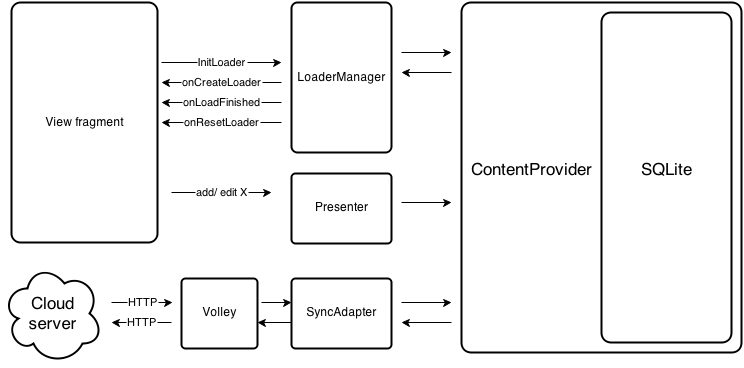
\includegraphics[width=\textwidth]{ch/architecture/fig/arch_app_overview.png}
\caption{Overview of how data is accessed.}
\label{fig:archAppOverview}
\end{figure}

ContentProviders contain a lot of boilerplate code and are time consuming to code. However, the upsides to using a ContentProvider far outweigh the downsides. ContentProviders used with a LoaderManager results in a view that is automatically updated when data changes, without bothering the UI thread.

\subsection{Business logic}
After defining a uniform access model to the database, the issue of where to place the actual business logic (data manipulation) must be tackled. Keeping the business logic in one place makes changing data manipulation logic a lot easier, avoids the issue of keeping track of where every data operation is defined in the view, and the bug bug free.

The team decided to use the pattern Model-View-Presenter (MVP). MVP is a Model-View-Controller (MVC) derivative~\cite{mvc}. All business logic is handled in presenter classes, between the views and models. Through this uniform access, all logic applied to data preservation (server synchronization), and data control can be handled in one place. How the presenter accesses data can be seen in figure~\ref{fig:archAppOverview}.

By using the full MVP pattern, the view is easy to update when data changes. In our case that was not needed since all data is accessed through a ContentProvider. The Presenters only handle the manipulation of the models and commits the changes to the database. The current implementation can easily be extended to use the complete pattern if it is needed in another iteration of the app.  

\begin{figure}[H]
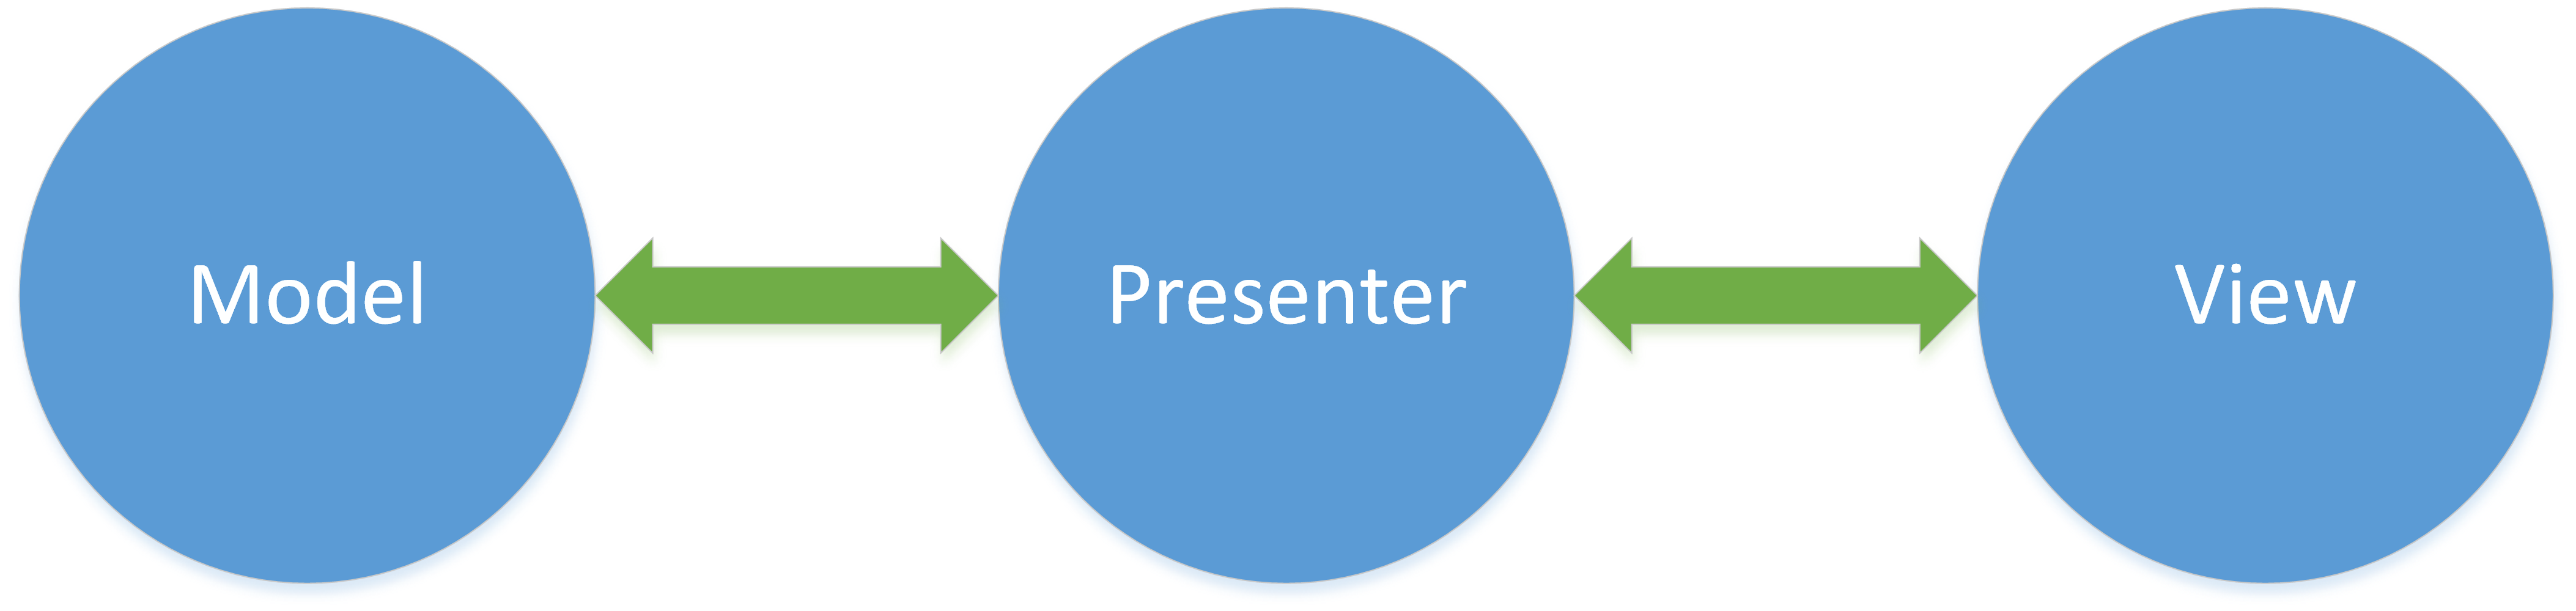
\includegraphics[width=\textwidth]{ch/architecture/fig/mvp.png}
\caption{MVP}
\label{fig:mvp}
\end{figure}

\subsection{User authentication}
The app is designed with the ability to synchronize data to the server. Our server, as explained in chapter~\ref{sec:arch_server}, exposes a restful API were data can be backed up.

The first challenge that arises with data synchronization is that the user must be identified as a unique and authorized user. Authentication is done with OAuthV2.0 and, for the time being, the third party authenticator is Facebook and session data is maintained with the FacebookSDK for Android. 
%For the moment this is not entirely true to how it is done now. Some shortcuts were done to have a working system. But the main authentication architecture is made.

The next case is how to handle the session data from Facebook. The Android system has its own account architecture. Working with this architecture requires the app to register a AbstractAccountAuthenticator~\cite{androidAccount} class in the AndroidManifest. The AbstractAccountAuthenticator is generic and can be made to create accounts for all types of services. The token and other related data (Facebook id) returned from Facebook is stored in the account and can accessed when necessary.

Other OAuthV2.0 authentication providers can also be used (Twitter, Google, your own private OAuthV2.0 authenticator, etc). 

%For the time being only the Facebook user id is used to authenticate the user to our server.

\subsection{Server communication}
Communication with the server is done with the framework ''Volley''. It is created by Google and the source code resides within AOSP (Android Open Source Project). It is made to make communication with restful endpoints easier.

Data synchronization is done by using Androids built in SyncAdapter. The SyncAdapter is a self-contained process that fetches and delivers all new data to and from the server. 

The SyncAdapter is registered to a specific account on the Android system. The account will then provide the session data that will identify the user to the server. How the session data was acquired was explained in the previous section. For the time being only the users Facebook id is as authentication with the server. 

\todo{This is not secure in any way. But changing this to use the session token, and make the server authenticate the user based on the token is an relatively easy improvement to implement. - FLYTT TIL FURTHER}

Communication with the database is still done through a ContentProvider, as seen in figure~\ref{fig:archAppOverview}. Since the changes will affect the URI, the view will get the new data and be rendered again automatically if the the app is running.

The algorithm for how data synchronization is done is showed as pseudo code in code snippet~\ref{fig:algorithm_sync}.\\

%Pseudo code for the sync

\noindent\begin{minipage}{\textwidth}
\begin{lstlisting}[caption={Algorithm for the synchronization flow}, label={fig:algorithm_sync}]
lastSync <- Last synchronization time stamp from account
now <- Current time in Unix epoch

localDataModels <- Get all local changes after lastSync

serverDataModels <- Get all server changes after lastSync

sendLocalModelsToServer(localDataModels)

saveModelsToLocalDB(serverDataModels)

if no errors
  accountLastSync = now
\end{lstlisting}
\end{minipage}

The algorithm is straightforward and will retry data synchronization until it succeeds. The reason for this is that the synchronization timestamp will only be updated when everything goes well. 

\todo{TIL FURTHER - 
If the error checking fails and the last synchronization timestamp fails, then data will be lost. 
This is not a perfect approach to synchronization, \todo{what? ->}but acceptable within the time frame that it was needed.} 

SyncAdapters can be configured to run when Android feels it has time to run them. This is when the processor is not busy and WiFi Internet connection is available. It can also be forced to run on regular intervals.

\subsection{Keeping the code clean}
Other long running operations, for example the rendering of the graph, will block the main thread if it is not implemented correctly. To avoid the main thread to be blocked in those cases, AsyncTask is used. AsyncTask is helpful when making asynchronous code that will update the view when finished.

\todo{ DETTE KAN NOK FJERNES -
\todo{Thereafter code written must generally continue to avoid doing wrong operations on the main thread. Forgetting to do this properly is easy. fix please, skjønner lite} To enforce the proper use of this threading, Android has a tool named StrictMode~\cite{androidStrictMode}. It can be tweaked to monitor the UI thread and check for file operations, network access and other problems. The penalty for breaking these defined rules can be set to emit a stack trace or kill the app. Having StrictMode configured while coding makes discovering bad implementation choices easier. 
}

%The app will follow standard Android design guidelines regarding the user interface design.
